\chapter{Use case: Lattic ECP5}
We will apply our algorithm to map virtual FPGAs to the concrete Lattice ECP5 FPGA. An image of this FPGA on an evaluation board is shown in Figure \ref{fig:evaluationboard}. This FPGA's architecture consists of `tiles' of different types in a grid pattern. Each of these tiles has an associated x- and y-coordinate in the grid system and is (generally) topologically the same as tiles of the type elsewhere in the grid. There exists I/O tiles which function is to retrieve and send data from outside the FPGA, DSP tiles that perform signal processing calculations, tiles that only provide routing structure, RAM tiles and tiles that are internally used for clock management and configuration.

The structure of an ECP5 FPGA is shown in Figure \ref{fig:ecp5architecture}. This figure shows the grid/tile structure of the ECP5 along with specific components from the electrical engineering domain. The largest portion of the grid structure are logic tiles that contain 8 LUTs and 8 registers (or flip-flops (FF)), bundled in 4 modules. We will focus on this type of tile to find homeomorphisms. We used Project Trellis\cite{todo} to obtain graphs of both an individual tile and of collections of adjacent tiles.

The virtual FPGA we aim to emulate on this board (which we will call \textit{VirBoard}) is one that, like the ECP5 consists of a tile-like structure with no wires spanning no more than a single tile. Because of this limitation, a student may freely drag-and-drop functionality in the virtual environment without worrying about implicitly overlapping connections. Each tile in this virtual FPGA has significantly less functionality than one of the ECP5. It has a single in- and output at each wind direction that may be connected in various ways, a 2-bit LUT and an 1-bit register. A graph model of VirBoard is shown in Figure \ref{fig:virboard}.

\begin{figure}
\centering
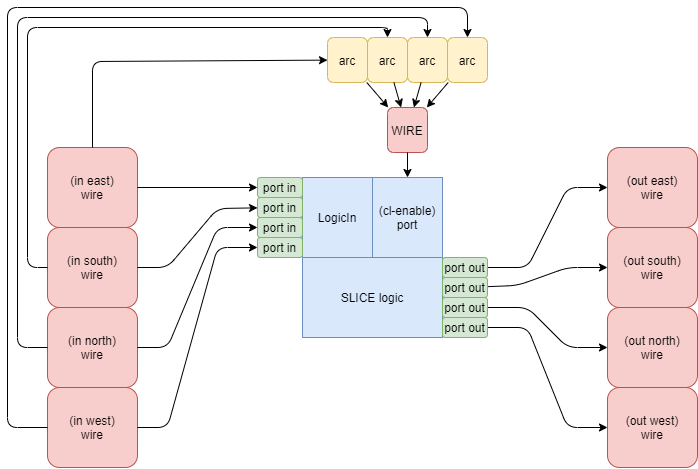
\includegraphics[width=0.8\textwidth]{images/virtualFPGA.png}
\caption{A graph model of a single cell of the virtual FPGA aimed to emulate on the Lattice ECP5}
\label{fig:virboard}
\end{figure}	


\begin{figure}
\centering
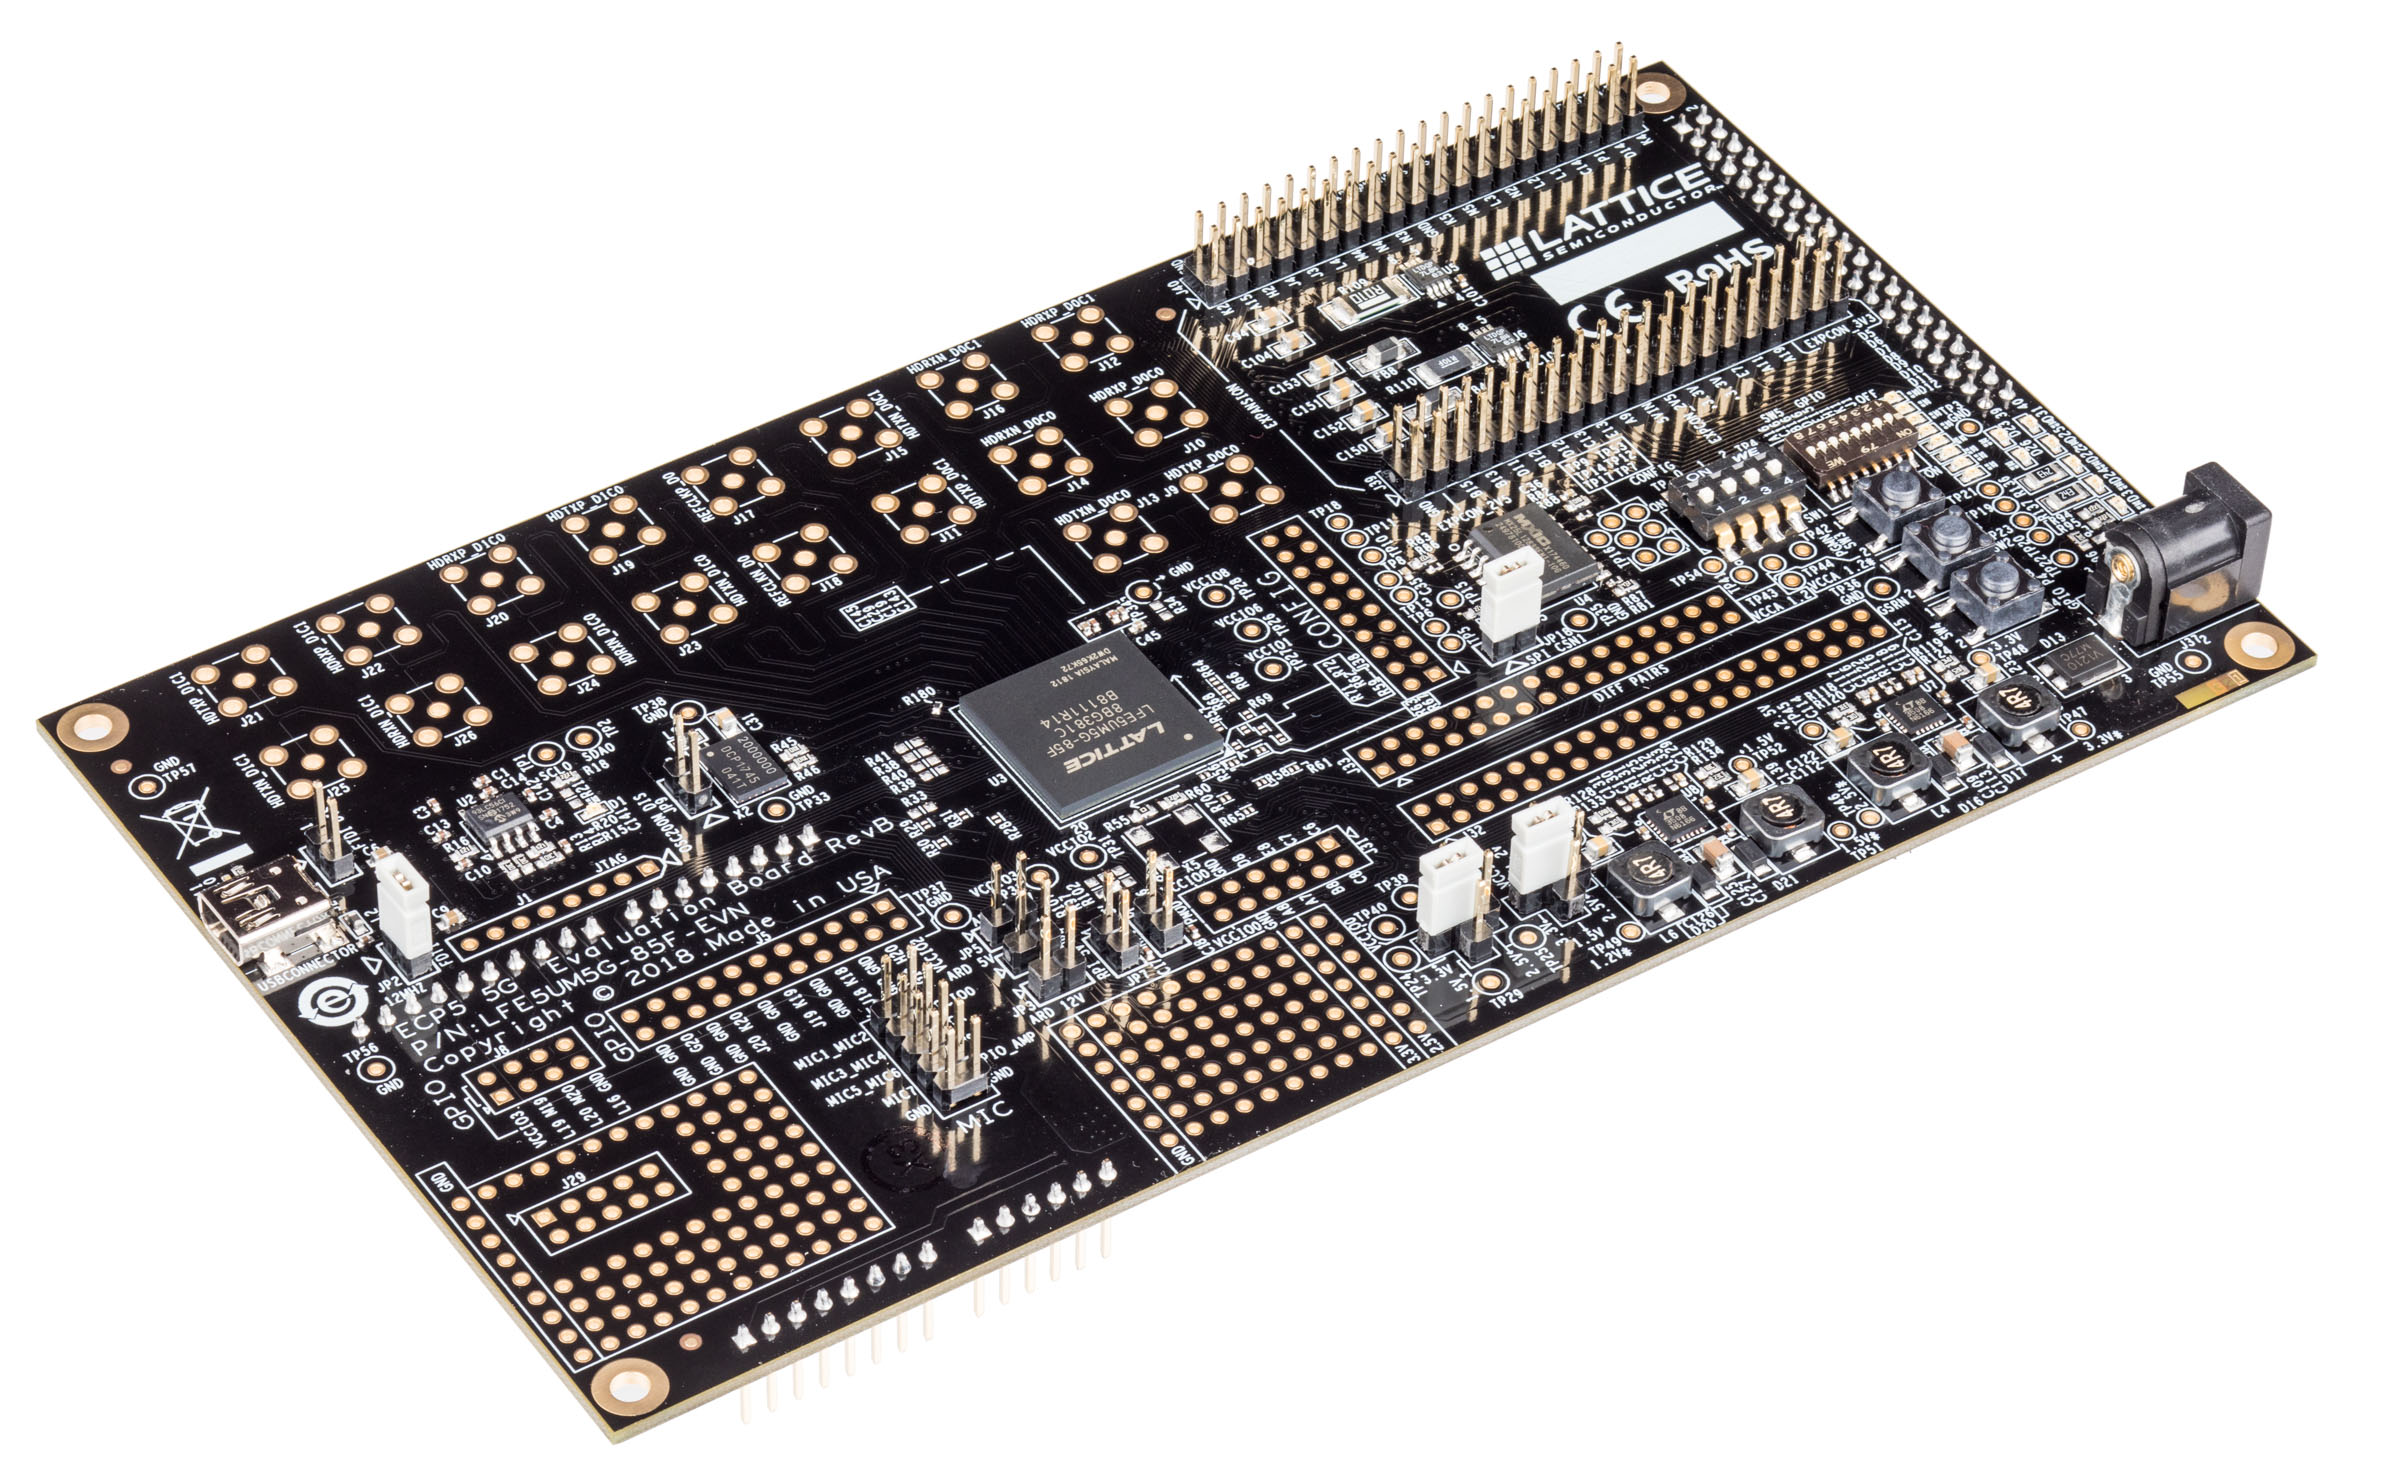
\includegraphics[width=0.5\textwidth]{images/ECP5.png}
\caption[Evaluation board of the LFE5UM5G-85F FPGA: a variant of the ECP5.]{Evaluation board of the LFE5UM5G-85F FPGA: a variant of the ECP5.\footnotemark}
\label{fig:evaluationboard}
\end{figure}
\footnotetext{\texttt{http://www.latticesemi.com/products/developmentboardsandkits/ecp5evaluationboard}, accessed July 10th 2020}	





